\documentclass[conference]{IEEEtran}
\IEEEoverridecommandlockouts
\usepackage{cite}
\usepackage{amsmath,amssymb,amsfonts}
\usepackage{graphicx}
\usepackage{textcomp}
\usepackage{xcolor}
\usepackage{url}
\DeclareMathOperator{\sg}{sg}
\DeclareMathOperator{\clip}{clip}
\newcommand{\R}{\mathbb{R}}
% Generated from unrounded supplied CSV values.
\newcommand{\ABSnormal}{65.19}
\newcommand{\ABSfog}{51.07}
\newcommand{\ABSsnow}{49.19}
\newcommand{\ABSmean}{50.13}
\newcommand{\BaseSnow}{45.67}
\newcommand{\BaseMean}{48.46}
\newcommand{\ABSnowGain}{3.52}
\newcommand{\ABMeanGain}{1.67}
\newcommand{\ABNormalLoss}{0.26}
\newcommand{\ABFogLoss}{0.19}
\newcommand{\PriorNormal}{65.87}
\newcommand{\PriorFog}{52.52}
\newcommand{\PriorSnow}{48.73}
\newcommand{\PriorMean}{50.62}
\newcommand{\PriorGain}{2.16}
\newcommand{\ABPriorSnowGain}{0.46}
\newcommand{\ABPriorMeanLoss}{0.49}

\pdfinfo{/Title (Evidence Routing and Supported Residuals for Cooperative LiDAR-Radar Perception)
/Author (Anonymous Authors)
/Subject (Cooperative perception with evidence routing and supported residuals)
/Keywords (cooperative perception, LiDAR-radar fusion, adverse weather)}

\begin{document}

\title{Evidence Routing and Supported Residuals for Cooperative LiDAR--Radar Perception}
\author{\IEEEauthorblockN{Anonymous Authors}}
\maketitle

\begin{abstract}
Cooperative perception depends on the quality of the local features that agents share. In adverse weather, missing LiDAR returns call for complementary evidence, whereas spurious returns call for suppression. We introduce DEER and SBR to separate these decisions from the support and amplitude of radar-based corrections. DEER learns independent missing and spurious scores from traceable point deletion and injection, then uses detached scores to route features while retaining each available modality. SBR selects local measured radar donors with a null option and bounds the resulting residual by observation support and current feature amplitude. Detection supervision learns the correction without a feature teacher. Seven configurations use a common 20-epoch, single-seed V2X-R protocol, with Snow held out from training and model selection. The joint model improves Snow Vehicle 3D average precision (AP3D) at intersection over union (IoU) 0.7 from \BaseSnow\ to \ABSsnow\ percent and the Fog/Snow mean by \ABMeanGain\ percentage points, with Normal/Fog decreases of \ABNormalLoss/\ABFogLoss\ points. A multiplicative type prior achieves the highest weather mean, \PriorMean\ percent. The joint design is strongest at strict 3D overlap in held-out Snow, while type-dependent amplitude modulation improves average weather performance.
\end{abstract}

\begin{IEEEkeywords}
cooperative perception, LiDAR--radar fusion, adverse weather, evidence routing, bounded residual
\end{IEEEkeywords}

\section{Introduction}
Cooperative perception extends an agent's sensing coverage by exchanging features across connected vehicles. Attentive aggregation, heterogeneous interactions, and selective communication improve this exchange~\cite{opv2v,v2xvit,where2comm}. Yet collaboration also distributes local measurement errors: an agent that shares corrupted features can degrade the joint detector. Preparing reliable local features is therefore a central part of cooperative perception.

Adverse weather poses two distinct problems for LiDAR: attenuation removes returns, while backscatter adds spurious returns~\cite{fog,snow}. A single suppression gate conflates these effects. It can reduce clutter but cannot supply missing evidence. Radar offers complementary measurements, although sparse coverage leaves some regions without a useful donor. A local fusion module must decide both how to route degraded observations and where radar can support a correction.

We address these decisions with DEER and SBR, inserted before a shared cooperative backbone. DEER learns independent missing and spurious scores from traceable point perturbations and uses them as detached routing signals. Positive modality gains preserve available evidence. SBR then selects nearby measured radar donors, including a null donor, and predicts a residual constrained by measured support and current feature scale. This separation gives degradation evidence, donor selection, and correction magnitude distinct roles. The detector learns the signed update directly, without a normal-feature teacher.

Our contributions are threefold:
\begin{itemize}
\item We introduce degradation-specific feature routing with independent deletion/injection supervision, detached type control, and retained modality gains. A current-amplitude descriptor preserves scale information in the normalized control path.
\item We formulate radar-guided correction with explicit spatial and amplitude constraints: local measured donors, a null option, a hard support mask, and a channelwise bound. The module operates before the common cooperative aggregation stage.
\item We evaluate seven configurations under a fixed training and selection protocol. The joint design gains \ABSnowGain\ percentage points in held-out Snow AP3D at IoU 0.7 and \ABMeanGain\ on the Fog/Snow mean; the controls reveal how routing, residual repair, and type conditioning affect the weather tradeoff.
\end{itemize}

\begin{figure*}[t]
\centering
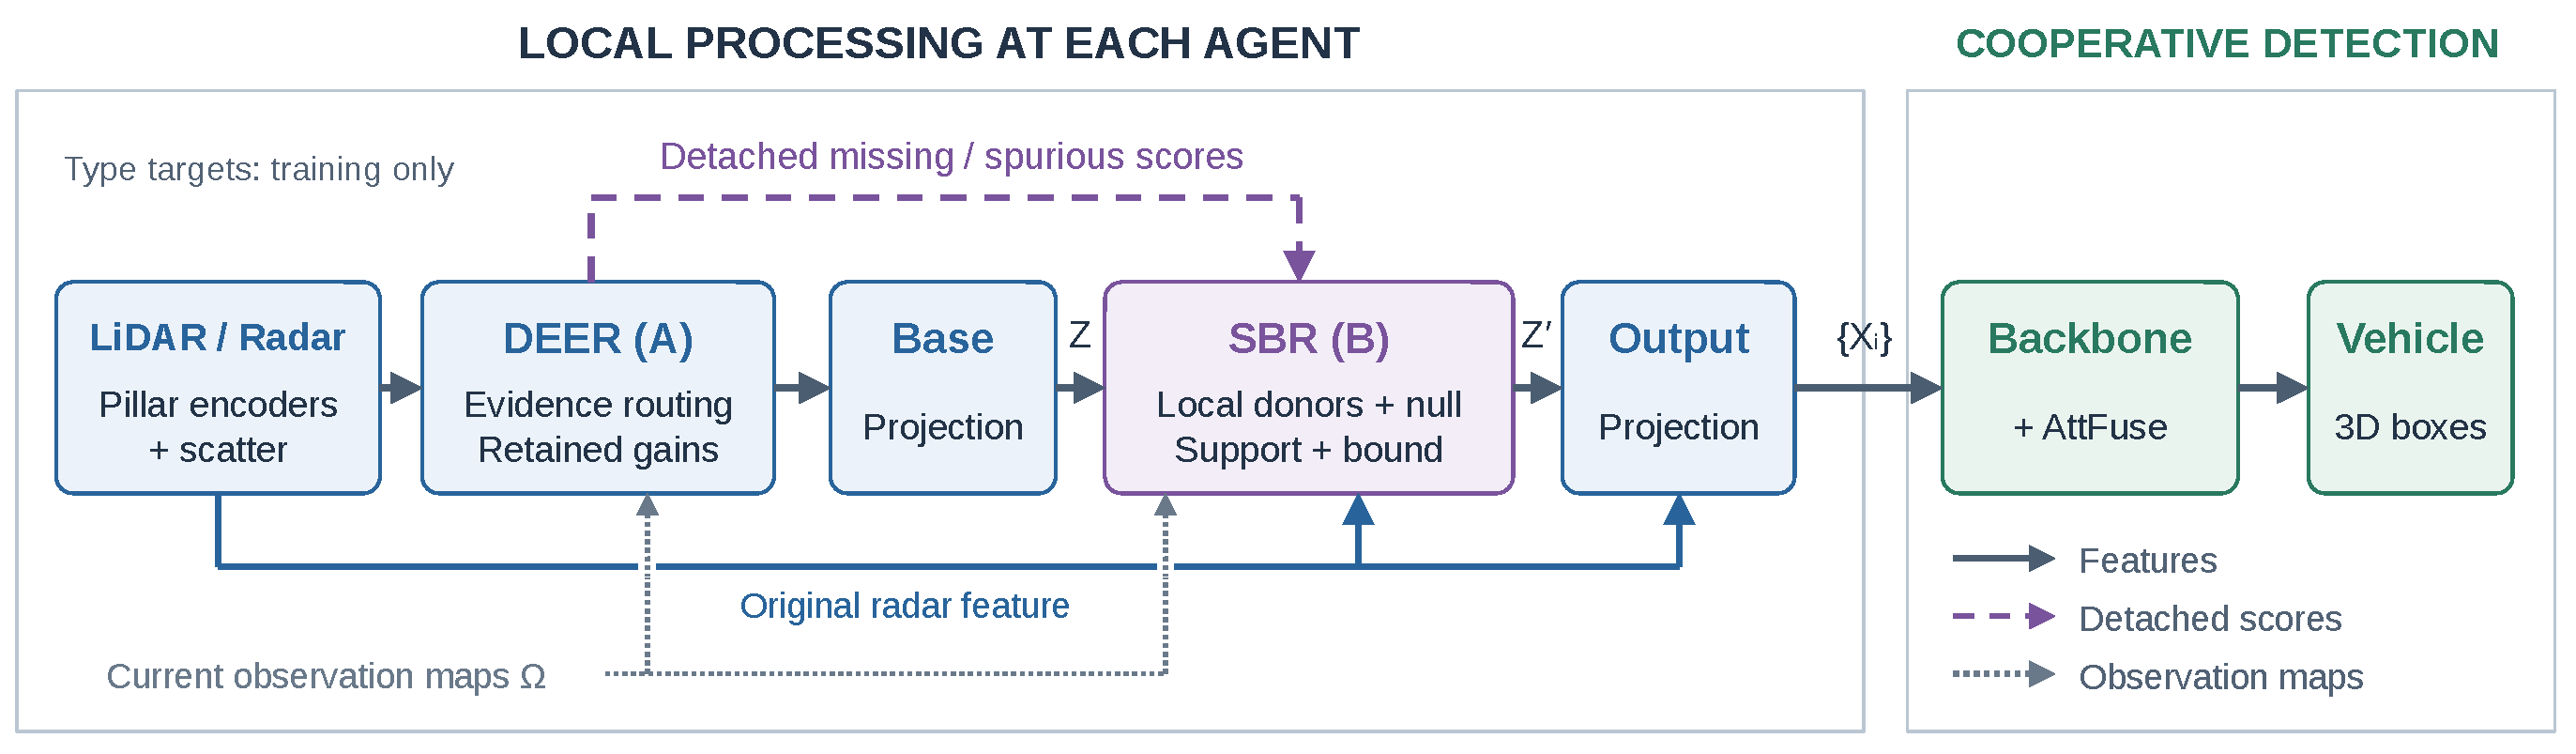
\includegraphics[width=\textwidth]{figures/architecture.pdf}
\caption{DEER and SBR prepare local features before cooperative detection. DEER routes LiDAR/radar features using detached missing/spurious evidence; SBR adds a radar-supported, amplitude-bounded residual. Solid arrows carry features, and the dashed arrow carries detached type scores. The dotted paths supply current observation maps; the lower solid path carries the original radar feature. All configurations share the radar bypass, output projection, backbone, and detection head. Type targets supervise training only.}
\label{fig:architecture}
\end{figure*}

\section{Related Work}
\subsection{Cooperative Three-Dimensional Perception}
OPV2V uses attentive intermediate fusion~\cite{opv2v}, V2X-ViT models heterogeneous inter-agent and spatial interactions~\cite{v2xvit}, and Where2comm selects transmitted regions through spatial confidence~\cite{where2comm}. CoAlign addresses pose errors with agent--object pose graphs and multiscale fusion~\cite{coalign}. Our method targets the local multimodal representation supplied to cooperation, while retaining the same aggregation stage and dataset poses across configurations.

\subsection{Weather-Aware LiDAR--Radar Fusion}
Physical weather models distinguish LiDAR attenuation from added returns~\cite{fog,snow}. L4DR combines foreground-aware radar filtering, shared-pillar information exchange, and gated fusion~\cite{l4dr}. V2X-R applies radar-conditioned denoising diffusion with a noise-masked reference-feature loss~\cite{v2xr}. HRCP couples opposite-modality sigmoid gates with channel-attentive residual enhancement and hybrid collaboration~\cite{hrcp}. DEER adds explicit provenance supervision for two degradation types; SBR makes measured radar support and current feature amplitude enforceable constraints on a directly predicted residual. These mechanisms distinguish our local processing from generic gating and residual enhancement.

\subsection{Reliability and Correction Support}
RAF supervises camera reliability and uses calibration-aware local matching for camera, LiDAR, and radar fusion~\cite{raf}. Our point-cloud model instead predicts controlled deletion/injection fractions and separates routing evidence from correction support. In SBR, null attention governs donor acceptance, a hard mask fixes where corrections are permitted, and an amplitude bound limits their size. These controls act at different stages of the same update.

\section{Method}
\subsection{Problem Definition}
For each agent $i$, current LiDAR and radar clouds are $P_i^L\in\R^{N_i^L\times4}$ and $P_i^R\in\R^{N_i^R\times4}$. Points contain coordinates and the source framework's red-channel scalar divided by 255, rather than calibrated velocity. Using supplied poses and calibration, the loader projects points once onto the ego grid and retains up to five agents within 70~m, including the ego. The detector outputs scored ego-frame Vehicle boxes with seven geometric parameters. Inputs exclude RGB pixels, weather-label color channels, provenance IDs, and reference features.

Separate pillar encoders and scatter operations~\cite{pointpillars} produce $F_i^L,F_i^R\in\R^{C\times H\times W}$, with $C=64$, $H=200$, and $W=704$. For each modality, the ten-channel observation tensor $\Omega$ records point count, occupancy, geometric field-of-view (FOV) validity, sensor-relative distance, and a broadcast availability flag $v_i^m\in\{0,1\}$. Counts enter the control encoder as $\log(1+\cdot)$; distance is divided by the bird's-eye-view (BEV) range diagonal. Occupancy is measured after geometric filtering and before voxel sampling; validity includes accepted boundary cells. Empty cells and unavailable frames remain distinct, and both retain the sample and its ground-truth (GT) boxes. Below, $b$ indexes a grid cell.

\subsection{Overall Architecture and Feature Units}
Fig.~\ref{fig:architecture} shows the insertion point between scatter and the common cooperative backbone.


Suppressing the agent index where unambiguous, the shared local path is
\begin{align}
Z_0 &= \Phi_{\mathrm{base}}([F^L,F^R]), \label{eq:base}\\
X &= \Phi_{\mathrm{out}}([Z',F^R]),\qquad
\widehat{\mathcal B}=\mathcal H(\mathcal C(\{X_i\}_{i=1}^n)), \label{eq:shared}
\end{align}
Here, $Z'$ is the corrected local feature, $\mathcal C$ is the multiscale AttFuse backbone, and $\mathcal H$ is the detection head; brackets concatenate channels. The bias-free pointwise projection $\Phi_{\mathrm{base}}$ maps $2C$ channels to $C$, and $\Phi_{\mathrm{out}}$ maps $2C$ to $2C$. Initialized at $[I,0]$ and $I$, both remain trainable in all configurations. S0 also shares the original radar bypass.

For any feature $F$, let $U(b)$ mark valid occupied cells and $\sg$ denote stop-gradient. The implemented per-agent, per-channel root-mean-square (RMS) operator $s=\mathcal R(F,U)$ is
\begin{align}
e_c&=\frac{\sum_b U(b)\sg(F_c(b))^2}{\max(\sum_b U(b),1)},\nonumber\\
\bar s&=\clip\!\left(\sqrt{C^{-1}\textstyle\sum_c e_c},\epsilon,M\right),\nonumber\\
s_c&=\clip\!\left(\clip(\sqrt{e_c},0.1\bar s,10\bar s),\epsilon,M\right), \label{eq:rms}
\end{align}
with $\epsilon=10^{-3}$ and $M=10^3$. This detached operator uses current observations, with a positive numerical floor for empty support. It normalizes control inputs and correction units; detection features and the radar bypass retain their learned units.

\subsection{DEER: Missing and Spurious Evidence Routing}
\subsubsection{Independent targets and predictions}
On a Normal training slot, the controlled deletion/injection process tracks the source identities of original LiDAR points. For each geometrically filtered cell, let $N_{\mathrm{ref}}$, $N_{\mathrm{del}}$, $N_{\mathrm{obs}}$, and $N_{\mathrm{inj}}$ count reference, deleted, observed, and injected points. The targets are
\begin{equation}
y_{\mathrm{miss}}=\frac{N_{\mathrm{del}}}{\max(N_{\mathrm{ref}},1)},\qquad
y_{\mathrm{spur}}=\frac{N_{\mathrm{inj}}}{\max(N_{\mathrm{obs}},1)}. \label{eq:targets}
\end{equation}
The validity masks are $U_{\mathrm{miss}}=\mathbf1[N_{\mathrm{ref}}>0]$ and $U_{\mathrm{spur}}=\mathbf1[N_{\mathrm{obs}}>0]$. Deletion and injection can coexist; unknown cells are masked. Targets use recorded source events, not changes in total point count. Unperturbed Normal observations have zero targets on valid occupied cells. Fog type targets are masked because their point-origin labels are unverified. Normal raw points provide training labels only.

Compute $s_L=\mathcal R(F^L,U_L)$ and $s_R=\mathcal R(F^R,U_R)$ on valid measured occupancy. The control representation is
\begin{align}
a_{\mathrm{amp}}&=[\log(1+s_L),\log(1+s_R)],\nonumber\\
E&=f_E\!\left(W_C[F^L/s_L,F^R/s_R,\Omega]+W_Aa_{\mathrm{amp}}\right). \label{eq:evidence}
\end{align}
Here $W_C$ projects $2C+10$ channels to 16 with bias. Bias-free $W_A$ projects $2C$ amplitude values to 16 and broadcasts them spatially, adding 2,048 parameters. The encoder uses SiLU, a 16-channel depthwise $3\times3$ convolution, SiLU, a $16\!\to\!16$ pointwise convolution, and SiLU. Separate two-channel pointwise heads predict type and route logits; independent sigmoids yield $d_{\mathrm{miss}}$ and $d_{\mathrm{spur}}$.

\subsubsection{Detached control and retained gains}
Learned route logits $h_L(E),h_R(E)$ receive type biases:
\begin{equation}
\ell_L=h_L(E)-\sg(d_{\mathrm{spur}}),\qquad
\ell_R=h_R(E)+\sg(d_{\mathrm{miss}}). \label{eq:route}
\end{equation}
For an available modality, define
\begin{equation}
\begin{aligned}
a_m&=\frac{v^m\exp(\ell_m)}{\sum_{k\in\{L,R\}}v^k\exp(\ell_k)},\\
g_m&=v^m[1+\alpha(2a_m-1)],
\end{aligned}\label{eq:gain}
\end{equation}
where $\alpha=0.5$. If both modalities are unavailable, weights and gains are set to zero. The routed representation is
\begin{equation}
Z_A=\Phi_{\mathrm{base}}([g_LF^L,g_RF^R]). \label{eq:routed}
\end{equation}
An available branch retains gain in $[0.5,1.5]$; an unavailable branch stays zero. Zero type-head weights/biases and compensated route-head biases initialize both gains to one, or to 1.5 for a sole available branch. Stop-gradient blocks detection gradients through type outputs, while both objectives train the shared encoder.

The descriptor in~\eqref{eq:evidence} restores amplitude information removed by normalization. Control N1 replaces it with occupied channel mean divided by the same RMS, preserving projection size and initialization.

\subsection{SBR: Observed Support and Bounded Residual Repair}
\subsubsection{Local donors and rejection}
SBR receives $Z=Z_A$ with A enabled and $Z=Z_0$ otherwise. The donor set $\mathcal K(b)$ contains measured radar cells within 0.8~m, checked by occupancy, FOV validity, and frame availability. On the 0.4~m grid, this gives 13 disk offsets within a $5\times5$ window.

The scale $s=\mathcal R(Z,U_L\lor U_R)$ uses the union of available valid occupancies. If the unguarded overall RMS of $Z$ is at most $\epsilon$ and radar is present, $s$ falls back to the current occupied radar RMS $s_R$. This permits radar correction when the LiDAR-led base feature is zero. Let $\widehat Z=Z/s$ and $\widehat R=F^R/s_R$.

Bias-free pointwise projections produce $q=Q\widehat Z$ and $k=K\widehat R$ in eight channels; $h_{\varnothing}$ is a zero-initialized affine $C\!\to\!1$ projection. The unit-ball map $\nu(x)=x/\max(\lVert x\rVert_2,1)$ gives real-donor scores
\begin{align}
t_u(b)&=2\nu(q(b))^\top\nu(k(u)),\quad u\in\mathcal K(b),\nonumber\\
t_{\varnothing}(b)&=h_{\varnothing}(\widehat Z(b))+\log\max(|\mathcal K(b)|,1). \label{eq:donorlogits}
\end{align}
Real scores lie in $[-2,2]$. A softmax over the valid candidates and always-valid null donor yields $\pi$. The normalized donor feature and hard support mask are
\begin{equation}
\widehat D(b)=\sum_{u\in\mathcal K(b)}\pi_u(b)\widehat R(u),\quad
S_R(b)=\mathbf1[|\mathcal K(b)|>0]. \label{eq:donor}
\end{equation}
The null feature is zero, and its mass is retained when summing real donors. The count term in~\eqref{eq:donorlogits} gives null mass $1/2$ when all uncorrected logits are zero and candidates exist. Without a candidate, null mass is one and $\widehat D=0$.

\subsubsection{Correction and explicit bound}
Let $h_A$ indicate that A supplies scores, and let $o_L$ be LiDAR occupancy. SBR's residual network reads
\begin{align}
r&=f_B([\widehat Z,\widehat D,\sg(d_{\mathrm{miss}}),\sg(d_{\mathrm{spur}}),o_L,S_R,h_A]),\nonumber\\
\Delta_c(b)&=S_R(b)\rho s_c\tanh(r_c(b)),\quad Z'=Z+\Delta, \label{eq:residual}
\end{align}
where $\rho=0.25$. The residual network uses a $2C+5\!\to\!16$ pointwise projection, SiLU, a depthwise $3\times3$ convolution, SiLU, and a $16\!\to\!C$ pointwise output. Without A, type scores and $h_A$ are zero; without B, $Z'=Z$.

The construction guarantees $\Delta=0$ where $S_R=0$ and $|\Delta_c(b)|\leq\rho s_c$ everywhere. A zero-initialized final layer starts with an identity update. The mask governs output support; null attention controls donor evidence but allows a residual where real support exists.

N2 tests an additional amplitude prior by multiplying~\eqref{eq:residual} by
\begin{equation}
G_A=0.25+0.75\max(\sg(d_{\mathrm{miss}}),\sg(d_{\mathrm{spur}})). \label{eq:prior}
\end{equation}
AB uses type scores as inputs only; N2 additionally applies this multiplier.

\subsection{Joint Training and Losses}
The detection loss combines focal classification (parameters 0.25 and 2) with twice smooth-$L_1$ regression (transition $1/9$). Regression sums seven anchor-relative codes with a sine yaw difference. Each sample's sums are divided by its positive-anchor count, clamped to one, and averaged across cooperative samples. Regression uses positive anchors; classification excludes ignored anchors.

For a mask $U$, $\langle V\rangle_U$ sums masked entries over all agents, cells, and applicable channels in the microbatch, divided by the broadcast mask sum clamped to one. With $n_i$ marking an unperturbed Normal agent slot, the auxiliary losses are
\begin{align}
\mathcal L_{\mathrm{type}}&=\sum_{t\in\{\mathrm{miss},\mathrm{spur}\}}\langle\operatorname{BCE}(d_t,y_t)\rangle_{U_t},\nonumber\\
\mathcal L_{\mathrm{size}}&=\langle(\Delta/\sg(s))^2\rangle_{S_R},\qquad
\mathcal L_{\mathrm{id}}=\langle|\Delta/\sg(s)|\rangle_{n_iS_R},\nonumber\\
\mathcal L&=\mathcal L_{\mathrm{det}}+0.1\mathcal L_{\mathrm{type}}
 +0.001\mathcal L_{\mathrm{size}}+0.01\mathcal L_{\mathrm{id}}. \label{eq:loss}
\end{align}
Binary cross-entropy operates on logits. Empty masks and inactive modules contribute zero. Fixed loss weights train the signed correction through detection, penalize its squared size on supported cells, and encourage identity on unperturbed Normal support. Training uses no reconstruction or feature-teacher loss.

At inference, the same feature path recomputes current RMS scales with fixed weights and batch-normalization (BN) statistics, then decodes and suppresses boxes. Perturbations and auxiliary targets are used only during training.

\section{Experiments}
\subsection{Experimental Setup}\label{sec:setup}
\subsubsection{Data and weather}
We evaluate on the simulated V2X-R dataset~\cite{v2xr}. Table~\ref{tab:data} gives the verified inventory, including 8,083 training samples. Sensor frames belong to cooperative samples and are not counted as independent examples.

\begin{table}[b]
\caption{Actual Split Inventory and Fixed Vehicle Ground Truth}
\label{tab:data}
\centering
\begin{tabular}{|l|r|r|r|}
\hline
Split & Coop. samples & Sensor frames & Fixed GT \\
\hline
Train & 8,083 & 24,088 & 69,757 \\
Validation & 829 & 3,041 & 6,414 \\
Test & 3,166 & 10,598 & 30,296 \\
\hline
\end{tabular}
\end{table}

We use the supplied paired Normal/Fog/Snow clouds, with unchanged radar. The weather versions are \texttt{\_fog\_0.060} and \texttt{\_snow\_2.5\_2.0}. During training, each agent uses Fog with probability $3/7$ and Normal otherwise, indexed deterministically by seed, epoch, sample, and agent. Snow is held out from training, validation, and model selection.

All groups apply the same provenance augmentation to Normal slots with probability 0.5: independently delete original points with probability 0.2 and inject $\lceil0.05N\rceil$ copies of sampled originals, including the scalar field. Offsets have isotropic directions and uniform radii in $[0.075,0.3]$~m. Injected points pass through the same self-mask, FOV, and range filters. The resulting deletion/injection fractions provide traceable supervision.

\subsubsection{Configurations and implementation}
Table~\ref{tab:variants} defines seven configurations built on the shared pillar/AttFuse detector in Fig.~\ref{fig:architecture}. S0 is the internal baseline. SUP retains the observation encoder, type loss, augmentation, and residual penalties, but uses ordinary gating and a residual from current normalized radar features. It removes type control, local donor attention, hard output support, and the $\tanh$ bound; penalties still use the common support mask. This approximately capacity-matched control tests the structured design as a whole.

\begin{table}[t]
\caption{Completed Configurations; Shared Protocol in Sec.~\ref{sec:setup}}
\label{tab:variants}
\centering
\begin{tabular}{|l|p{0.77\columnwidth}|}
\hline
Group & Local mechanism or controlled change \\
\hline
S0 & Shared detector and radar bypass; A/B disabled. \\
\hline
A & DEER only. \\
\hline
B & SBR only; no A predictions or type inputs. \\
\hline
AB & Joint model; detached types enter B as inputs. \\
\hline
SUP & Ordinary gating/residual control (Sec.~\ref{sec:setup}). \\
\hline
N1 & AB with occupied mean/RMS replacing the RMS descriptor; same size and initialization. \\
\hline
N2 & AB with the multiplicative type prior in~\eqref{eq:prior}; all other settings unchanged. \\
\hline
\end{tabular}
\end{table}

Pillars are $0.4\times0.4\times4$~m over $[-140.8,140.8)\times[-40,40)\times[-3,1)$~m, with up to 32 points each and 32,000/70,000 pillars per modality in training/evaluation. Backbone stages have 128/256/512 channels, each with a stride-2 $3\times3$ convolution and 3/5/8 stride-1 layers. AttFuse aggregates at each scale; upsampling produces three 128-channel maps for the classification/regression heads. Vehicle anchors are $3.9/1.6/1.56$~m in length/width/height, with $0/90$-degree headings and output stride 2. Assignment uses continuous stand-up BEV IoU: positive at 0.6 or above, negative below 0.45, and ignored otherwise, plus a positive-overlap best anchor per GT.

Geometric augmentation applies an $x$-axis world flip, rotation in $[-\pi/4,\pi/4]$, and scaling in $[0.95,1.05]$. Optional local branches use activation checkpointing during training.

\subsubsection{Training and selection}
Each group trains for 20 epochs and 20,200 optimizer updates with seed 17. FP32 microbatch 4 with two accumulation steps gives effective batch 8; incomplete effective batches are dropped. Runs use individual RTX 2080 Ti GPUs. S0 resumes an audited checkpoint at update 1,000 within the same total budget; other groups share initialization of common parameters. Adam uses learning rate 0.002, weight decay $10^{-4}$, and $\epsilon=10^{-10}$; the rate decreases tenfold at epochs 10 and 15.

Every epoch is validated on all 829 Normal and Fog samples. BN buffers are first reset and refitted by cumulative averaging over eight microbatches of four fixed training samples (32 samples total), drawn by uniform midpoint sampling from the epoch-0 Normal/Fog/provenance stream without geometric augmentation. Only BN statistics update; parameters and other modules remain fixed. BN uses $\epsilon=0.001$ and online momentum 0.01.

Selection maximizes mean Normal/Fog validation AP3D at IoU 0.7, retaining the earlier epoch for ties within $10^{-6}$. N1/N2 select epoch 18; all others select epoch 20. Selected weights and BN statistics are frozen across all three test conditions.

\subsubsection{Scoring}
We report Vehicle AP3D and BEV average precision (APBEV) at IoU 0.3/0.5/0.7 using global confidence ordering, one-to-one matching within each sample, and VOC2010 all-point interpolation. The fixed GT set retains boxes with ego-frame centers in $x\in[0,140)$~m and $y\in[-40,40)$~m and a camera-geometric FOV defined by calibration and image dimensions. GT acceptance is independent of point count; zero-target samples remain.

Postprocessing uses confidence floor 0.001, rotated BEV non-maximum suppression IoU 0.15, and at most 500 detections. All 21 tests cover 3,166 samples and 30,296 fixed GT boxes. The adverse-weather summary is
\begin{equation}
M_{\mathrm{weather}}=\tfrac12\left(\mathrm{AP3D}^{\mathrm{Fog}}_{0.7}+\mathrm{AP3D}^{\mathrm{Snow}}_{0.7}\right). \label{eq:weather}
\end{equation}
This Fog/Snow mean differs from the Normal/Fog validation selection score. AP is reported in percent; differences are percentage points calculated from unrounded CSV values.

\subsection{Detection Across Weather Conditions}
AB achieves the highest Snow AP3D at IoU 0.7 among the seven configurations: \ABSsnow\ percent, up \ABSnowGain\ points from S0 (Table~\ref{tab:main}). Its Fog/Snow mean improves by \ABMeanGain\ points, while Normal/Fog decrease by \ABNormalLoss/\ABFogLoss\ points. N2 leads Normal, Fog, and the weather mean, improving the latter by \PriorGain\ points over S0. AB leads N2 by \ABPriorSnowGain\ in Snow, whereas N2 leads AB by \ABPriorMeanLoss\ on the mean.

\begin{table}[t]
\caption{Test Vehicle AP3D at IoU 0.7 (\%; Higher Is Better). $M_{\mathrm{weather}}$ Is Defined in~\eqref{eq:weather}; $\Delta M$ Is Its Change from S0 in Percentage Points. Bold Indicates Column Maxima.}
\label{tab:main}
\centering
\begin{tabular}{|l|r|r|r|r|r|}
\hline
Group & Normal & Fog & Snow & $M_{\mathrm{weather}}$ & $\Delta M$ \\
\hline
S0 & 65.46 & 51.25 & 45.67 & 48.46 & +0.00 \\
A & 64.67 & 51.60 & 46.22 & 48.91 & +0.45 \\
B & 65.18 & 51.41 & 44.72 & 48.06 & -0.40 \\
AB & 65.19 & 51.07 & \textbf{49.19} & 50.13 & +1.67 \\
SUP & 64.84 & 51.36 & 46.24 & 48.80 & +0.33 \\
N1 & 64.37 & 51.03 & 48.69 & 49.86 & +1.40 \\
N2 & \textbf{65.87} & \textbf{52.52} & 48.73 & \textbf{50.62} & +2.16 \\
\hline
\end{tabular}

\end{table}

AB's Snow gain grows from 0.24 points at IoU 0.3 to 0.75 at 0.5 and \ABSnowGain\ at 0.7. The largest improvement therefore occurs under the strictest 3D overlap criterion, making high-overlap Snow detection the clearest benefit of the joint design.

\subsection{Module Interaction and Design Controls}
\subsubsection{Separate and joint modules}
Table~\ref{tab:factorial} compares S0, A, B, and AB. A improves the weather mean by 0.45 points; B decreases it by 0.40, including a 0.96-point Snow loss. Combining the modules raises Snow AP3D by 2.98/4.48 points over A/B and the weather mean by 1.22/2.07. The descriptive interaction is
\begin{equation}
I=\mathrm{AP}_{AB}-\mathrm{AP}_{A}-\mathrm{AP}_{B}+\mathrm{AP}_{S0}. \label{eq:interaction}
\end{equation}
The interaction is +3.93 points in Snow and $-0.69$ in Fog. The positive joint effect is thus concentrated in Snow: routing and supported correction together outperform either module alone in that condition.

\begin{table}[t]
\caption{Derived Four-Cell Effects at IoU 0.7 (Percentage Points). $I$ Is Defined in~\eqref{eq:interaction}; Values Are Derived from the Runs in Table~\ref{tab:main}.}
\label{tab:factorial}
\centering
\begin{tabular}{|l|r|r|r|r|}
\hline
Condition & A$-$S0 & B$-$S0 & AB$-$S0 & $I$ \\
\hline
Normal & -0.79 & -0.28 & -0.26 & +0.81 \\
Fog & +0.35 & +0.16 & -0.19 & -0.69 \\
Snow & +0.54 & -0.96 & +3.52 & +3.93 \\
$M_{\mathrm{weather}}$ & +0.45 & -0.40 & +1.67 & +1.62 \\
\hline
\end{tabular}

\end{table}

\subsubsection{Ordinary control SUP}
AB exceeds SUP by 2.96 points in Snow and 1.33 on the weather mean, with a 0.35-point Normal gain and a 0.29-point Fog loss. The structured routing/correction design therefore improves on ordinary gating and residual prediction under the same augmentation and type supervision.

\subsubsection{Amplitude descriptor N1}
AB exceeds N1 by 0.82 points in Normal, 0.04 in Fog, and 0.50 in Snow, with a 0.27-point gain on the weather mean. The RMS amplitude descriptor performs better than the equally parameterized occupied-mean/RMS alternative in all three conditions, with the smallest difference in Fog.

\subsubsection{Type-prior control N2}
N2 adds only the multiplier in~\eqref{eq:prior} to AB. Its higher Normal/Fog scores and weather mean show that explicit type-dependent amplitude modulation remains useful, while AB retains the strongest Snow AP3D. Type conditioning therefore offers a concrete design choice between strict-overlap Snow performance and average weather performance.

\subsection{Metric and Selection Sensitivity}
Table~\ref{tab:auxiliary} places the strict-overlap result in context. N2 leads Snow APBEV at IoU 0.7 (65.56 versus AB's 65.42), while SUP leads Snow AP3D at 0.3/0.5 (83.78/77.81 versus 82.87/77.37). The complete six-metric results for all three weather conditions accompany the paper.

\begin{table}[t]
\caption{Auxiliary Test AP (\%; Higher Is Better). Left: Snow AP3D at IoU 0.3/0.5; Right: APBEV at IoU 0.7 for Each Weather Condition. Bold Indicates Column Maxima.}
\label{tab:auxiliary}
\centering
\begin{tabular}{|l|r|r|r|r|r|}
\hline
 & \multicolumn{2}{c|}{Snow AP3D} & \multicolumn{3}{c|}{APBEV at IoU 0.7} \\
\cline{2-6}
Group & IoU 0.3 & IoU 0.5 & Normal & Fog & Snow \\
\hline
S0 & 82.64 & 76.61 & 77.59 & 62.99 & 63.86 \\
A & 83.17 & 77.18 & 77.20 & 63.61 & 64.87 \\
B & 82.73 & 76.14 & 76.71 & 62.62 & 62.63 \\
AB & 82.87 & 77.37 & 77.40 & 63.74 & 65.42 \\
SUP & \textbf{83.78} & \textbf{77.81} & \textbf{77.61} & 63.36 & 65.20 \\
N1 & 83.52 & 77.78 & 77.26 & 63.07 & 65.11 \\
N2 & 83.37 & 77.57 & 77.48 & \textbf{63.98} & \textbf{65.56} \\
\hline
\end{tabular}

\end{table}

AB's Normal/Fog validation mean is 49.54 versus S0's 49.15; SUP leads at 51.22. The corresponding test mean is 58.13 for AB and 58.36 for S0. These rankings differ from the Fog/Snow test mean, where N2 ranks first and AB second, because the conditions and splits differ. Selection remains fixed throughout.

\section{Discussion and Conclusion}
DEER and SBR separate degradation-aware routing from observation-supported correction. DEER turns independent missing/spurious supervision into retained modality gains; SBR turns measured radar support and current feature scale into explicit constraints on the residual. Together they improve Snow AP3D at IoU 0.7 by \ABSnowGain\ points and the Fog/Snow mean by \ABMeanGain\ over the shared baseline. The type-prior control achieves the highest weather mean, highlighting the value of tailoring correction strength to the target conditions.

The study uses one seed, 20 epochs, and one simulated dataset with unchanged radar. Small control differences and the descriptive interaction require repeated runs; SUP tests several mechanisms jointly. Same-protocol external baselines, real-road data, joint sensor degradation, and deployment-cost measurements are the next evaluation priorities.

% Balance the final bibliography columns without changing the IEEE type size.
\IEEEtriggeratref{7}
% Numeric IEEE references, in order of first citation, as in the supplied template.
% Only verified fields are included. Primary-source lookup URLs are recorded
% separately in evidence/reference_verification.json.
\begin{thebibliography}{00}
\bibitem{opv2v}
R. Xu, H. Xiang, X. Xia, X. Han, J. Li, and J. Ma, ``OPV2V: An open benchmark dataset and fusion pipeline for perception with vehicle-to-vehicle communication,'' in \emph{Proc. IEEE Int. Conf. Robotics and Automation (ICRA)}, 2022.

\bibitem{v2xvit}
R. Xu, H. Xiang, Z. Tu, X. Xia, M.-H. Yang, and J. Ma, ``V2X-ViT: Vehicle-to-everything cooperative perception with vision transformer,'' in \emph{Proc. European Conf. Computer Vision (ECCV)}, 2022.

\bibitem{where2comm}
Y. Hu, S. Fang, Z. Lei, Y. Zhong, and S. Chen, ``Where2comm: Communication-efficient collaborative perception via spatial confidence maps,'' in \emph{Advances in Neural Information Processing Systems}, vol. 35, 2022.

\bibitem{fog}
M. Hahner, C. Sakaridis, D. Dai, and L. Van Gool, ``Fog simulation on real LiDAR point clouds for 3D object detection in adverse weather,'' in \emph{Proc. IEEE/CVF Int. Conf. Computer Vision (ICCV)}, 2021.

\bibitem{snow}
M. Hahner \emph{et al.}, ``LiDAR snowfall simulation for robust 3D object detection,'' in \emph{Proc. IEEE/CVF Conf. Computer Vision and Pattern Recognition (CVPR)}, 2022, pp. 16364--16374.

\bibitem{coalign}
Y. Lu \emph{et al.}, ``Robust collaborative 3D object detection in presence of pose errors,'' in \emph{Proc. IEEE Int. Conf. Robotics and Automation (ICRA)}, 2023.

\bibitem{l4dr}
X. Huang \emph{et al.}, ``L4DR: LiDAR-4DRadar fusion for weather-robust 3D object detection,'' in \emph{Proc. AAAI Conf. Artificial Intelligence}, vol. 39, no. 4, 2025, pp. 3806--3814, doi: 10.1609/aaai.v39i4.32397.

\bibitem{v2xr}
X. Huang \emph{et al.}, ``V2X-R: Cooperative LiDAR-4D radar fusion with denoising diffusion for 3D object detection,'' in \emph{Proc. IEEE/CVF Conf. Computer Vision and Pattern Recognition (CVPR)}, 2025. [Online]. Available: \url{https://arxiv.org/abs/2411.08402v5}

\bibitem{hrcp}
Y. Yang, H. Zhang, W. Lu, Z. Zhang, C. Zhang, and X. Xu, ``Hybrid robust collaborative perception with LiDAR-4D radar fusion under adverse weather conditions,'' in \emph{Proc. IEEE/CVF Conf. Computer Vision and Pattern Recognition (CVPR)}, 2026, pp. 24237--24247.

\bibitem{raf}
H. Park, J. Jeong, and K.-J. Yoon, ``RAF: Reliability-aware fusion of camera, LiDAR, and 4D RADAR for robust 3D object detection in adverse weather,'' arXiv:2607.04587v1, 2026.

\bibitem{pointpillars}
A. H. Lang, S. Vora, H. Caesar, L. Zhou, J. Yang, and O. Beijbom, ``PointPillars: Fast encoders for object detection from point clouds,'' in \emph{Proc. IEEE/CVF Conf. Computer Vision and Pattern Recognition (CVPR)}, 2019, pp. 12697--12705.
\end{thebibliography}

\end{document}
